\documentclass[xcolor=pdftex,dvipsnames,table,mathserif,aspectratio=169]{beamer}
\usetheme{default}
\usetheme{metropolis}
\usepackage{minted}
\usepackage{mathtools}
\setbeamersize{text margin left=.3in,text margin right=.3in} 

\usepackage[english]{babel}
\usepackage{pgf,pgfarrows,pgfnodes,pgfautomata,pgfheaps}
\usepackage{amsmath,amssymb,setspace,centernot}
\usepackage[latin1]{inputenc}
\usepackage{pgf,tikz}
\usepackage[T1]{fontenc}
\usepackage{relsize}
\usepackage{pdfpages}
\usepackage[absolute,overlay]{textpos} 


\DeclareMathOperator*{\argmax}{arg\,max}
\DeclareMathOperator*{\argmin}{arg\,min}

\newcommand{\X}{\mathtt{X}}
\newcommand{\Y}{\mathtt{Y}}

%\newcommand{\R}{\mathbb{R}}
%\newcommand{\E}{\mathbb{E}}
%\newcommand{\V}{\mathbb{V}}
\newcommand{\p}{\mathbb{P}}
\newcommand*\df{\mathop{}\!\mathrm{d}}
\newcommand{\del}{\partial}


% imports
\usepackage{xargs}
\usepackage{xpatch}
\usepackage{etoolbox}
\usepackage{pdflscape}
\usepackage{booktabs}
\usepackage{threeparttable}
\usepackage[skip=0.2\baselineskip]{caption}

% command for inputting raw latex
\makeatletter
\newcommand\primitiveinput[1]{\@@input #1 }
\makeatother

% common table command
\newcommandx{\tablecontent}[4]{
    \begin{threeparttable}[!ht]
        \centering
        \caption{#3}
        \vspace{-1em}
        \footnotesize
        \begin{tabular}{#1}
            \primitiveinput{../tables/#2.tex}
        \end{tabular}
        \vspace{-0.2em}
        \begin{tablenotes}[flushleft]
            #4
        \end{tablenotes}
    \end{threeparttable}
}




% \usepackage{slashbox}
\title{ Advanced Panel Data:\\
Interpreting FE?}
\author{Chris Conlon }
\institute{NYU Stern }


\newcommand{\norm}[1]{\left\lVert#1\right\rVert}
\newcommand{\R}{\mathbb{R}}
\newcommand{\E}{\mathbb{E}}
\newcommand{\V}{\mathbb{V}}
\newcommand{\ol}{\overline}
%\newcommand{\ul}{\underline}
\newcommand{\pp}{{\prime \prime}}
\newcommand{\ppp}{{\prime \prime \prime}}
\newcommand{\policy}{\gamma}


\newcommand{\fp}{\frame[plain]}

\date{\today}

\begin{document}
\maketitle

\section*{Causal FE}

\begin{frame}
\frametitle{Recall the FE Assumptions}
\begin{align*}
y_{it} =  x_{it}'\beta + \eta_i + \varepsilon_{it}
\end{align*}
\vspace{-.7cm}
\begin{itemize}
\item $\eta_i$ is a \alert{fixed effect}.
\item To estimate everything consistently, we need $E[ \varepsilon_{it} | x_{it}, \eta_i]=0$
\item Mostly this is not true. Instead usually treat $\eta_i$ as a \alert{control variable} or \alert{nuisance parameter}.
\begin{itemize}
\item A nuisance parameter is one that we estimate but don't care about interpreting.
\item If we only care about $\beta$ then $\eta_i$ is a nuisance parameter.
\end{itemize}
\item With a control or nuisance parameter we only require that $E[ \varepsilon_{it} | \eta_{i}]=E[ \varepsilon_{it} | x_{it}, \eta_i]$ \alert{conditional mean independence}.
\item Once we condition on $\eta_i$ it is as if $\varepsilon_{it}$ and $x_{it}$ are uncorrelated.
\end{itemize}
\end{frame}


\begin{frame}{Causal FE}
\begin{itemize}
\item We can get away with conditional mean independence if we don't care about $\eta_i$.
\item But suppose that we care about $\widehat{\eta}_i$?
\begin{itemize}
\item Teacher FE
\item Physician/Hospital FE
\item Location/County FE
\end{itemize}
\item Suppose move someone from the $10th$ percentile to the $90th$ percentile
\begin{itemize}
\item This about the variance/second moment of $\eta_i$.
\end{itemize}
\end{itemize}
\end{frame}


\begin{frame}{Causal FE}
\begin{itemize}
\item Now we have to really believe $E[ \varepsilon_{it} | x_{it}, \eta_i]=0$
\item We should worry about the conventional \alert{omitted variable bias} problem.
\item Suppose there exists a variable $w_{it}$ so that:
\begin{eqnarray*}
y_{it} =  x_{it}'\beta +  w_{it}'\gamma + \eta_i + \varepsilon_{it}
\end{eqnarray*}
\item Recall the conditions for OVB
\begin{itemize}
\item $w_{it}$ is correlated with $x_{it}$
\item $w_{it}$ is a determinant of $y_{it}$
\end{itemize}
\item New one:  $w_{it}$ is correlated with $\eta_i$
\begin{itemize}
\item This is easy to satisfy!
\item $w_{it}$ needs to be uncorrelated with anything about the individual $i$.
\end{itemize}
\end{itemize}
\end{frame}



\begin{frame}{Example: Test Scores}
\begin{itemize}
\item Students $s$, Teachers $i$
\item Want to measure effect of \alert{Teachers} on \alert{Test Scores}
\begin{eqnarray*}
y_{is} = x_{is}' \beta  + \eta_i + \varepsilon_{is}
\end{eqnarray*}
\item We observe some features of students but not all of them (parent's education, household income, language spoken at home).
\item We also observe some school specific variables $w_{is}$ but not all of them (district spending per pupil, \% free lunch, etc.).
\item But we don't observe other things (jackhammering outside the classroom, which students have disruptive home lives,etc.).
\begin{itemize}
\item If the mean of those things varies across teachers $\rightarrow$ we are screwed!
\item Can't get an accurate estimate of $\eta_i$.
\end{itemize}
\end{itemize}
\end{frame}


\begin{frame}{Example: Test Scores}
We need a better design:
\begin{itemize}
\item We probably need random assignment of students to teachers.
\item Ideally we would be able to control for student and school unobservables.
\item Might want to see many students match with many teachers.
\end{itemize}
\end{frame}

\begin{frame}{Example: Test Scores}
Even random assignment is not enough:
\begin{align*}
y_{is} =  \eta_i + \varepsilon_{is}
\end{align*}
For each teacher the mean test score is:
\begin{align*}
\overline{y}_{i} =  \eta_i + \frac{1}{S_i} \sum_{s=1}^{S_i} \varepsilon_{is}
\end{align*}
\begin{itemize}
\item But $S_i \rightarrow \infty$ doesn't hold. So relative variance of $\eta_i$ and $\varepsilon_{is}$ matters.
\item People with large $\overline{y}_i$ may mostly be lucky (small $S_i$).
\item May want to apply \alert{shrinkage} estimator again.
\end{itemize}
\end{frame}



\begin{frame}{Example: Test Scores}
Even random assignment is not enough:
\begin{align*}
y_{is} =  \eta_i + \varepsilon_{is}
\end{align*}
For each teacher the mean test score is:
\begin{align*}
\overline{y}_{i} =  \eta_i + \frac{1}{S_i} \sum_{s=1}^{S_i} \varepsilon_{is}
\end{align*}
\begin{itemize}
\item But $S_i \rightarrow \infty$ doesn't hold. So relative variance of $\eta_i$ and $\varepsilon_{is}$ matters.
\item People with large $\overline{y}_i$ may mostly be lucky (small $S_i$).
\item May want to apply \alert{shrinkage} estimator again.
\end{itemize}
\end{frame}


\begin{frame}{Example: Test Scores}
\begin{align*}
y_{ist} = x_{ist}\beta +  \underbrace{\alert{\eta_i}+ \lambda_{it} +  \varepsilon_{ist}}_{u_{ist}}
\end{align*}
\begin{itemize}
\item Now residual $u_{ist}$ contains a teacher ``quality'' $\eta_i$ that we are interested in
\item $\lambda_{it}$ a ``classroom'' or teacher-year specific deviation.
\item Goal: think about a forecast of $y_{i,t+1} | \mathbf{y}_{t}$
\end{itemize}
\end{frame}


\begin{frame}{How ?}
Estimate $\hat{u}_{ist}$ and construct the following:
\begin{itemize}
\item Within classroom student variance: $\hat{\sigma}_{s}^{2}=\operatorname{Var}\left(u_{i s t}-\overline{u}_{it} \right)$
\item Auto-Covariance within teacher across years/classrooms: $\hat{\sigma}_{\eta}^{2}=\operatorname{Var}\left(\overline{u}_{it}, \overline{u}_{i,t+k} \right)$
\item Classroom Variance: $\hat{\sigma}_{\lambda}^{2}=\operatorname{Var} (u_{ist} ) - \hat{\sigma}_{\eta}^{2} -\hat{\sigma}_{s}^{2}$. 
\item Weight each classroom by its inverse variance ($n_{it}$ is students per classroom):
\begin{align*}
\begin{array}{c}
\overline{u}_{i}=  \sum_{t} w_{it} \overline{v}_{it}, \quad 
 w_{it} = \frac{h_{it}}{\sum_t h_{it}} \\
 h_{it} = \frac{1}{\operatorname{Var} (\overline{u}_{it} | \eta_i )}  = \frac{1}{\sigma_{\lambda}^2 + \frac{\sigma_{s}^2}{n_{it}}} 
\end{array}
\end{align*}
\item But $\overline{u}_{i}$ is still not the best \alert{forecast} estimate of $\eta_i$.
\end{itemize}
\end{frame}


\begin{frame}{How ?}
We want to further shrink our estimate $\overline{u}_{i}$ to account for the variance in our estimate:
\begin{align*}
\eta_i = \overline{u}_i \times \frac{\sigma_{\eta}^2}{\operatorname{Var} (\overline{u}_{i} )}
\end{align*}
\begin{itemize}
\item Where $\operatorname{Var} (\overline{u}_{i} )= \sigma_{\eta}^2 + \left(\sum_t h_{it} \right)^{-1} $
\item Idea: fraction of teacher variance explained by FE $\eta_i$ as opposed to $\lambda_{it}$ and student factors.
\item Shrinkage factor always $\leq 1$ and smaller for less precise estimates.
\item Hope: if teachers teach many students with similar scores, we have a precise estimate of $\eta_i$.
\end{itemize}
\end{frame}



\begin{frame}{Best Counties? (Chetty Hendren 2016 AER)}
\begin{center}
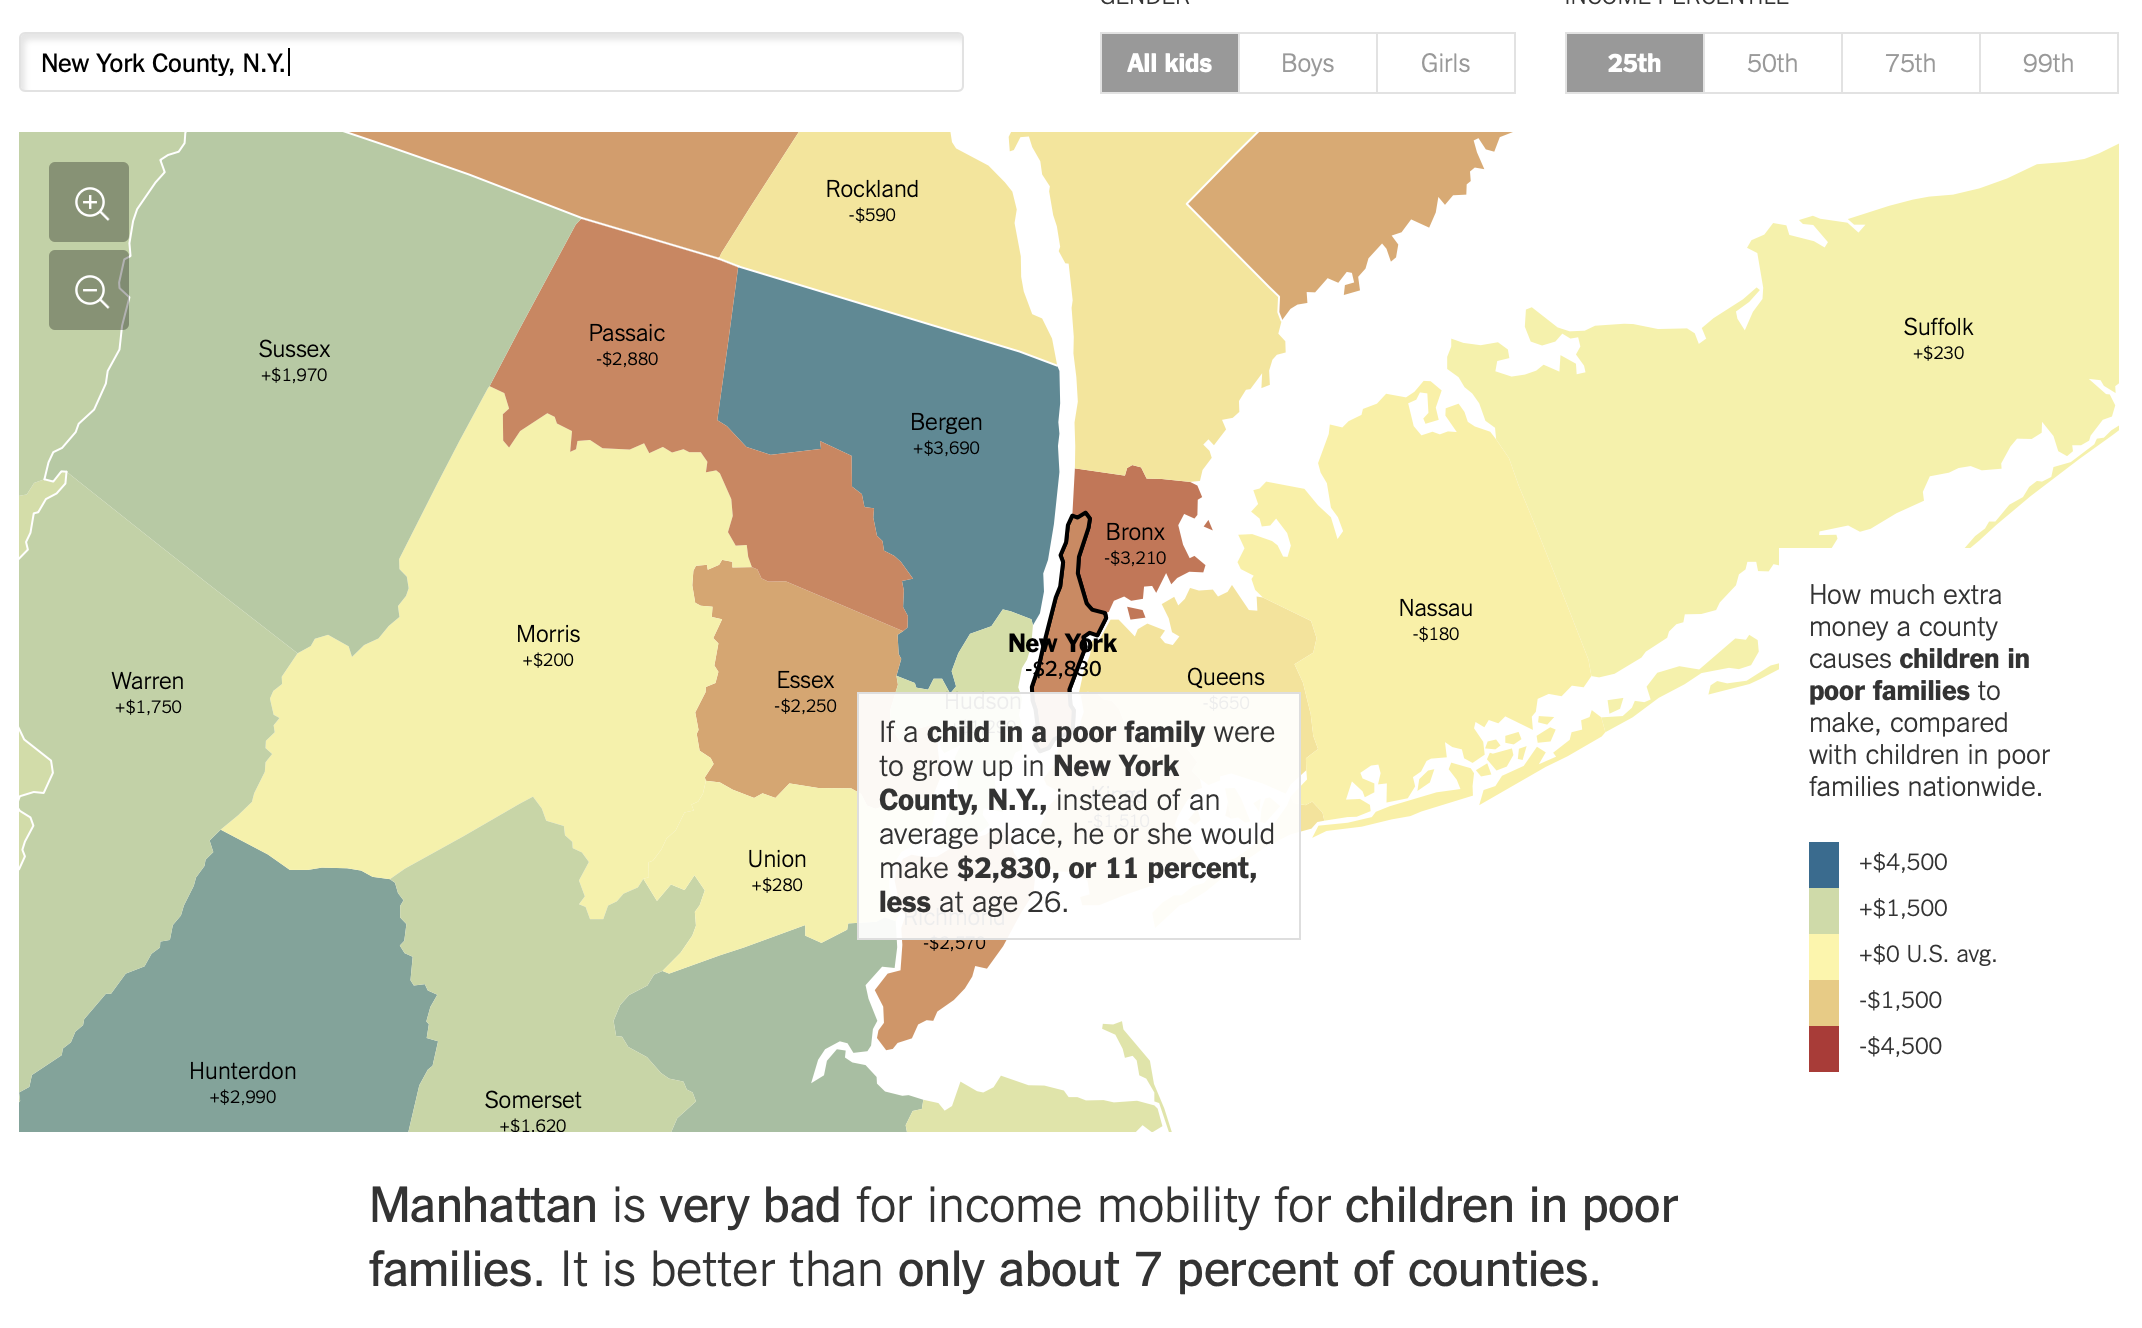
\includegraphics[width=4in]{./resources/chetty2.png}
\end{center}
\end{frame}


\begin{frame}{Best Counties?}
\begin{center}
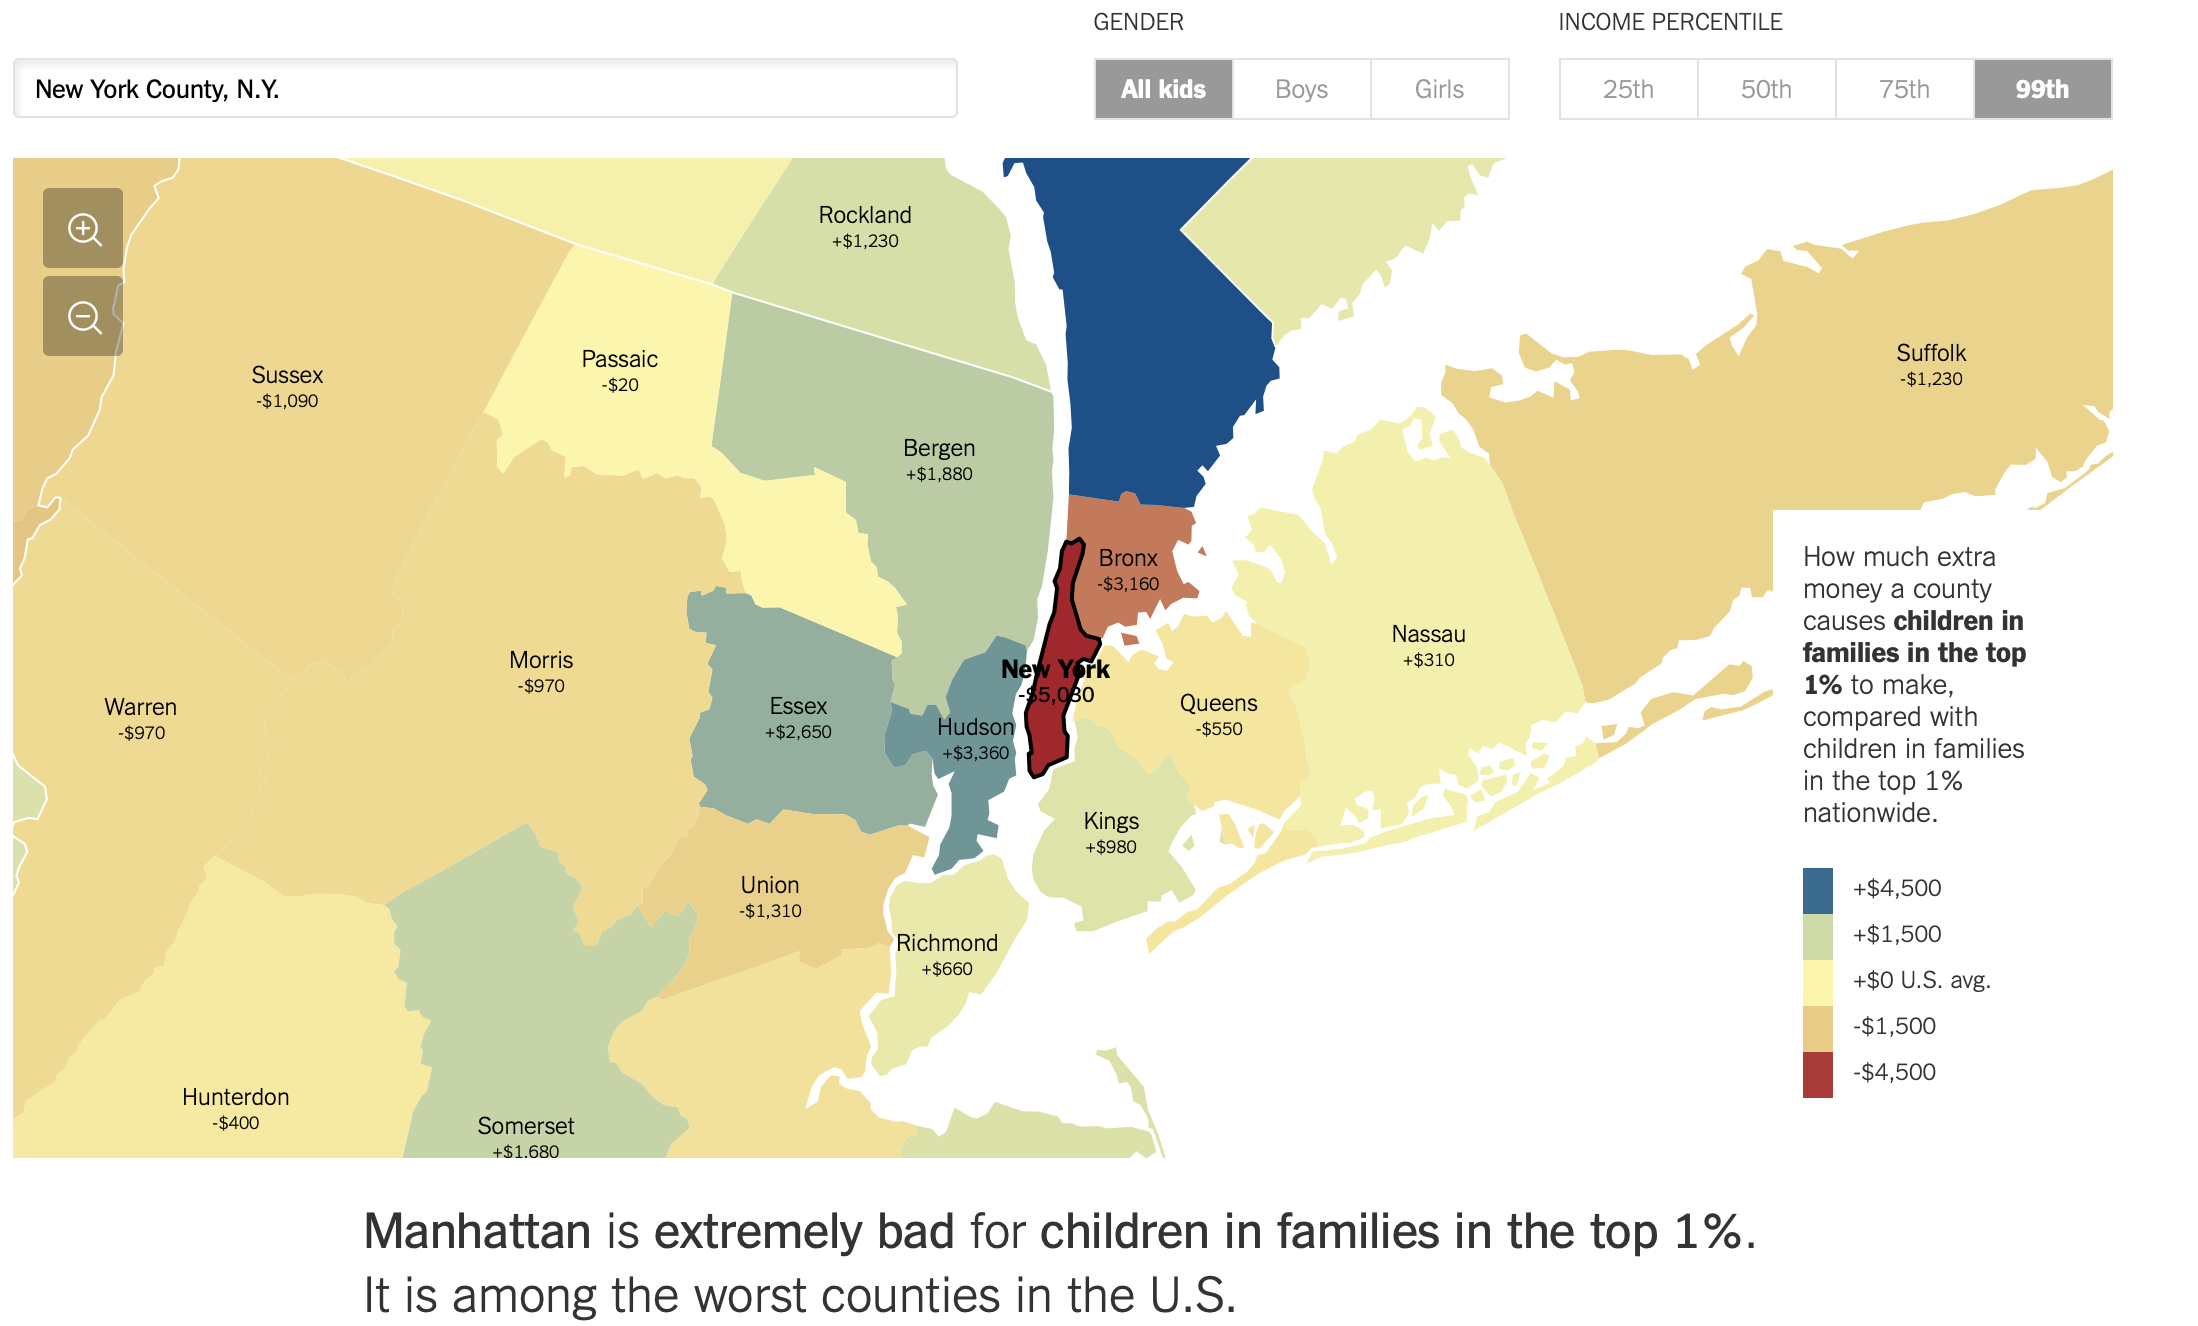
\includegraphics[width=4in]{./resources/chetty3.png}
\end{center}
\end{frame}

\begin{frame}{Best Counties?}
50,000 residents (and very few people move here).
\begin{center}
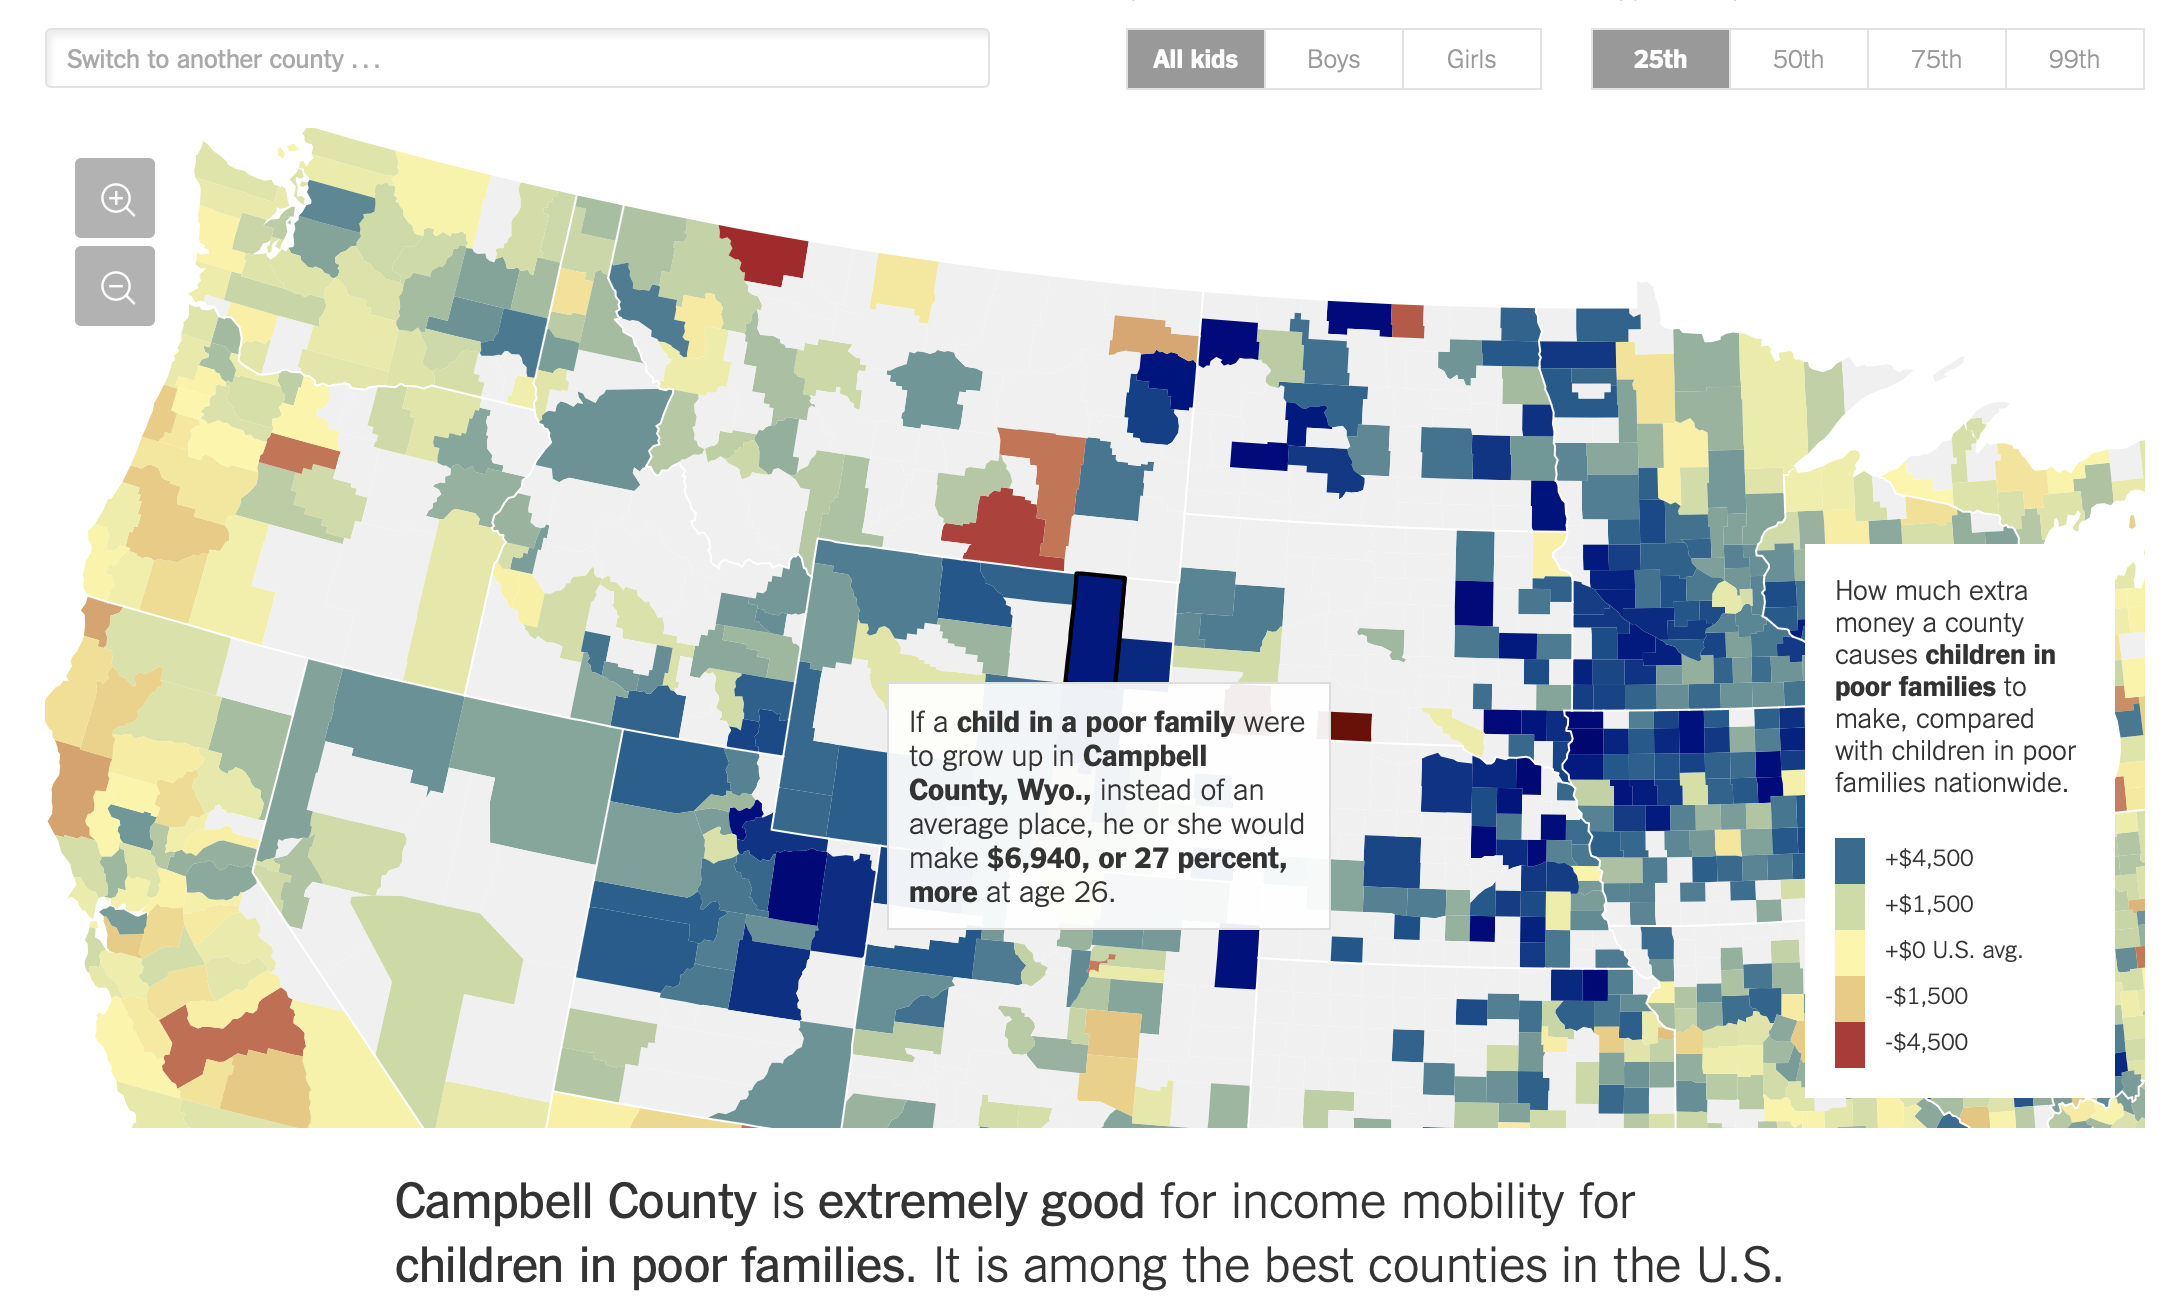
\includegraphics[width=4in]{./resources/chetty1.png}
\end{center}
\end{frame}


\begin{frame}{Time to move to Campbell County, WY?}
Less than 10\% of Campbell County residents graduated college (among worst in US):
\begin{center}
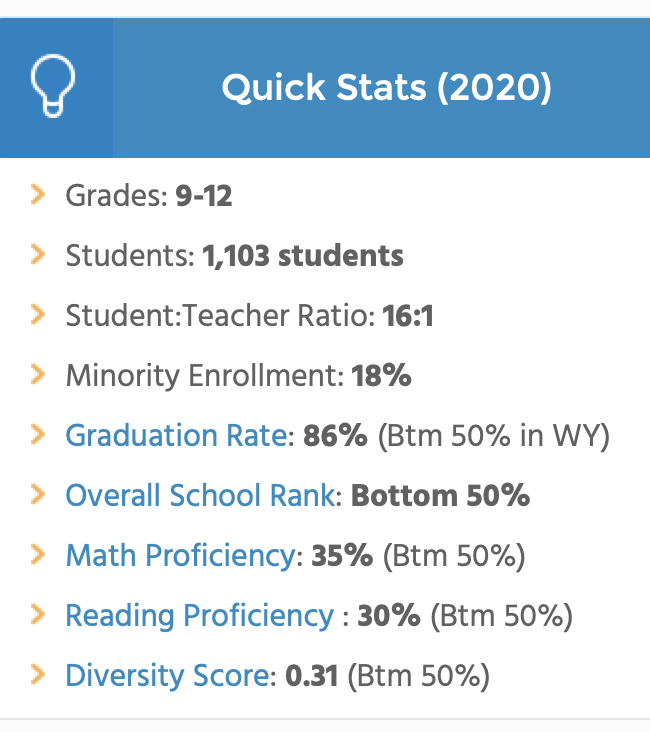
\includegraphics[width=2in]{./resources/chetty4.png}
\end{center}
\end{frame}


\begin{frame}{What's going on?}
Is Campbell county the land of opportunity?
\begin{itemize}
\item Or is it a small place that nobody moves to with very imprecisely measured FE $\gamma_i$?
\item Helped that people found coal in their backyards (literally)
\item If you moved there today would you still expect to do well?
\end{itemize}
This problem is endemic:
\begin{itemize}
\item Our ``best'' and ``worst'' teachers tend to be those who teach the fewest students.
\item Presumably FE are estimated with precision that is not equal.
\end{itemize}


\end{frame}



\begin{frame}{Healthcare Exceptionalism: Static Reallocation}
Is \alert{quality} (or productivity) correlated with \alert{market share}?
\begin{align*}
\ln \left(N_{h}\right)=\beta_{0}^{s}+\beta_{1}^{s} q_{h}+\gamma_{M}^{S}+\varepsilon_{h}^{s}
\end{align*}
\begin{itemize}
\item $N_h$ measures market size for hospital $h$
\item $\gamma_M^s$ are market FE
\item $q_h$ is measure of hospital quality
\item Goal: Is $\beta_1^s>0$ or not. $\beta_1^s<0$ is usually only Soviet countries or 1970's steel.
\item $\beta_1^s>0$ means allocation towards productive firms (or just returns to scale?)
\end{itemize}
\end{frame}

\begin{frame}{Healthcare Exceptionalism: Dynamic Reallocation}
\begin{align*}
\Delta_{h}&=\beta_{0}^{d}+\beta_{1}^{d} q_{h}+\gamma_{M}^{d}+\varepsilon_{h}^{d}\\
\Delta_{h}&=\frac{N_{h, 2010}-N_{h, 2008}}{\frac{1}{2}\left(N_{h, 2010}+N_{h, 2008}\right)}
\end{align*}
\begin{itemize}
\item $\beta_1^d>0$ means growth towards productive firms (not just returns to scale)
\item Same idea but now we capture \alert{dynamics}.
\item Patients may still be attracted to \alert{unobservables correlated with quality}.
\end{itemize}
\end{frame}


\begin{frame}{Healthcare Exceptionalism}
\begin{center}
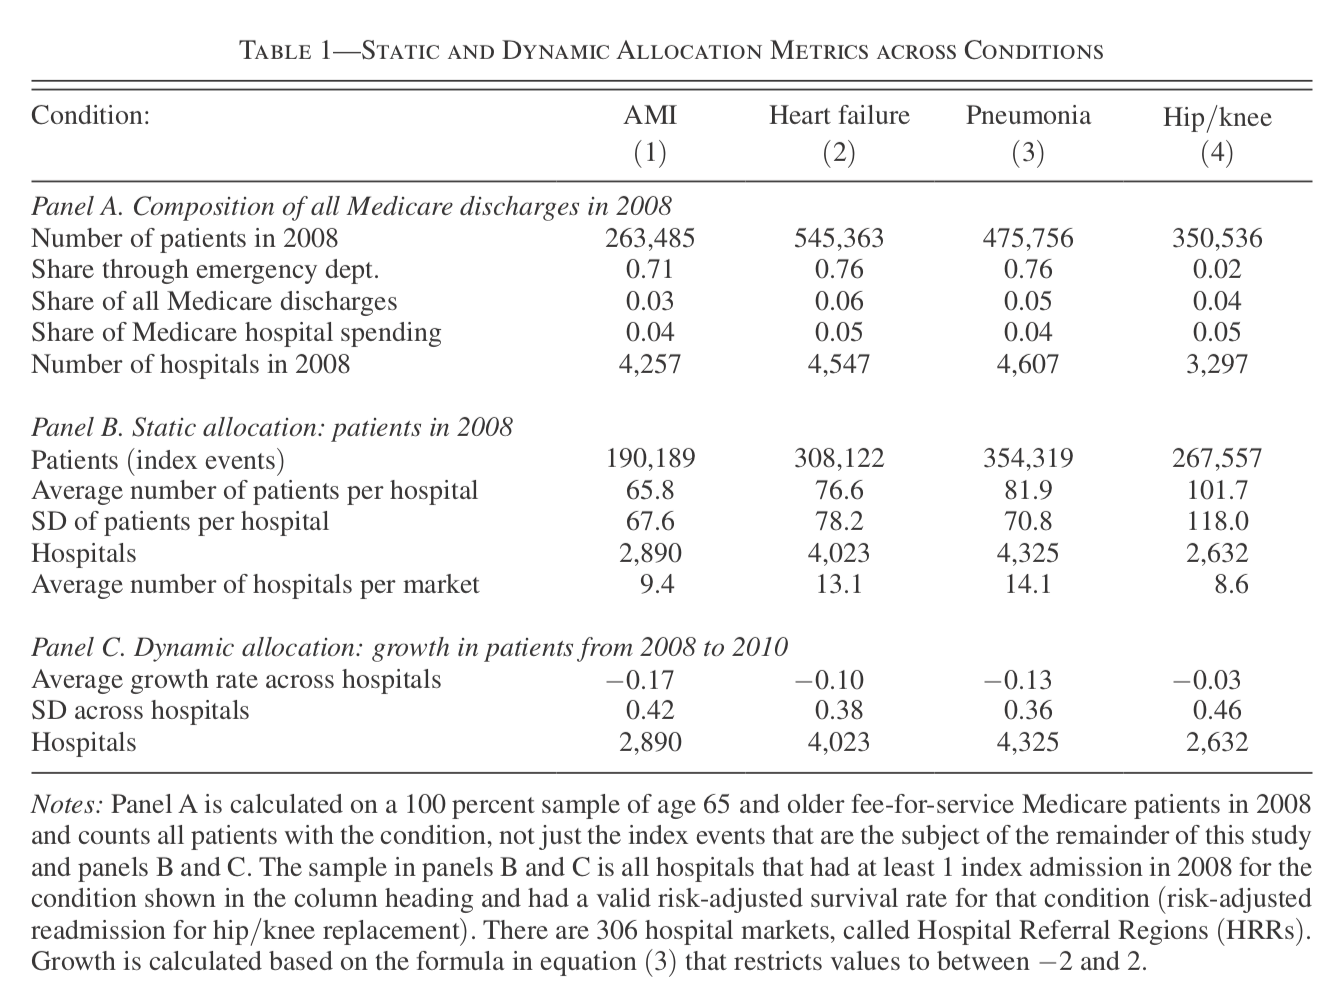
\includegraphics[width=4in]{./resources/hc1.png}
\end{center}
\end{frame}

\begin{frame}{Healthcare Exceptionalism}
\begin{center}
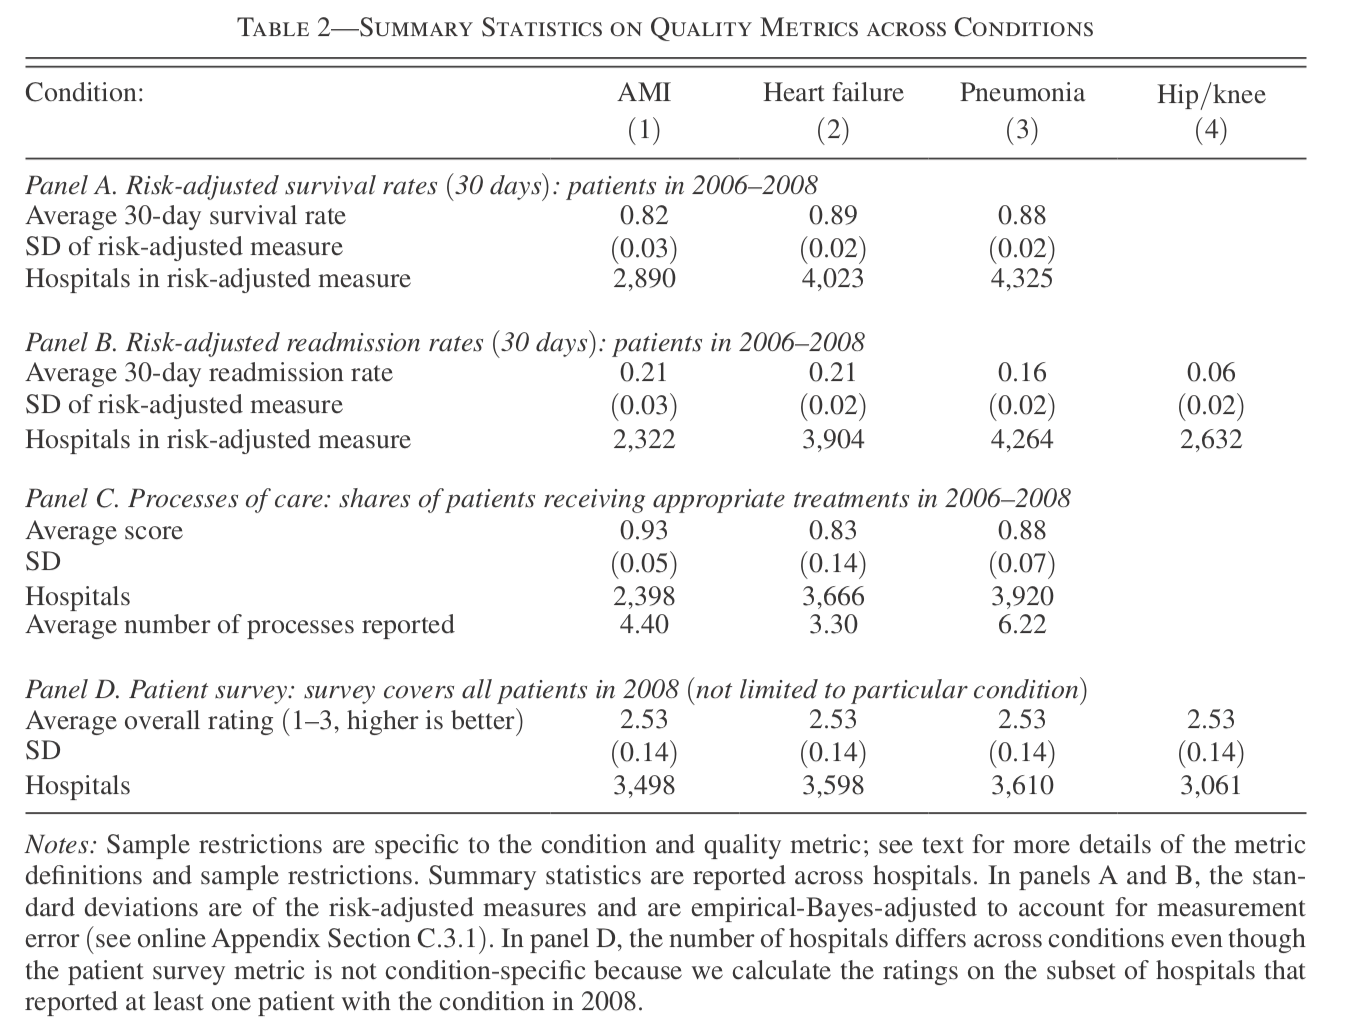
\includegraphics[width=4in]{./resources/hc2.png}
\end{center}
\end{frame}

\begin{frame}{Healthcare Exceptionalism}
\begin{center}
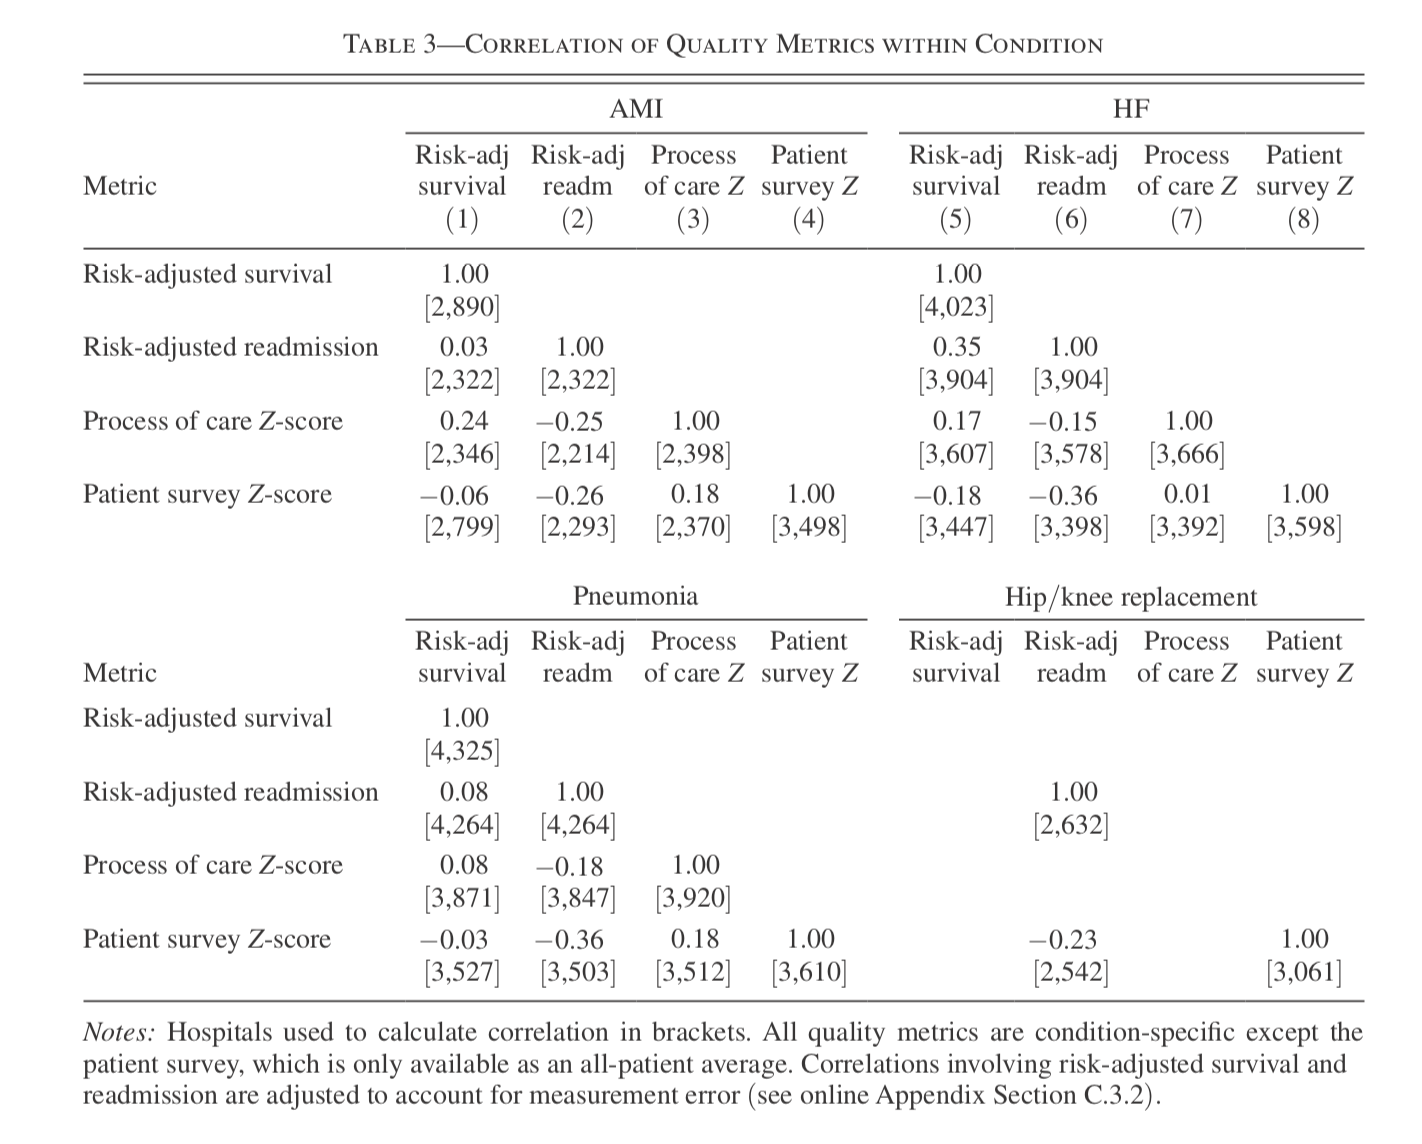
\includegraphics[width=4in]{./resources/hc3.png}
\end{center}
\end{frame}

\begin{frame}{Healthcare Exceptionalism}
\begin{center}
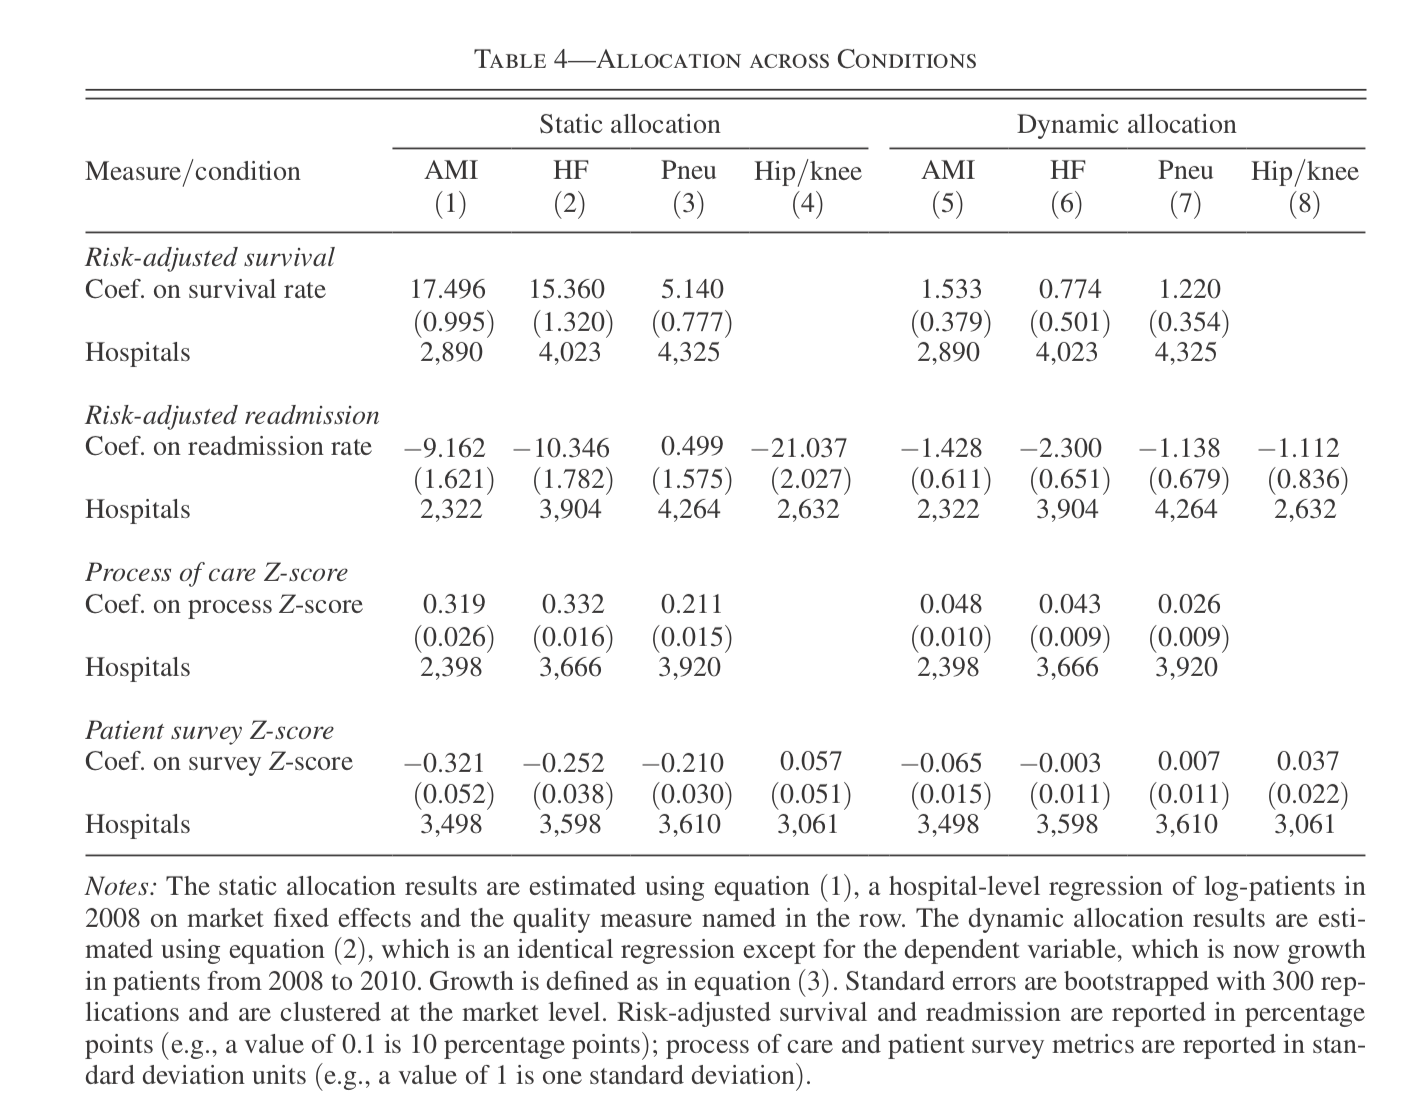
\includegraphics[width=4in]{./resources/hc4.png}
\end{center}
\end{frame}




\begin{frame}{Healthcare Exceptionalism: Production Function}
Hospital Production Function:
\begin{align*}
y_{p}^{s}=a_{h}+\sum_{k} \lambda_{k} r_{p k}+\mu x_{p}+\xi_{p}
\end{align*}
\begin{itemize}
\item $a_h$ is \alert{hospital productivity} (a FE) and variable of interest
\item $y_p$ is a patient outcome (survival-days, etc.)
\item $x_p$ are (log) hospital inputs
\item $r_{pk}$ are patient risk factors.
\item This has interpretation as a \alert{production function}. Why?
\end{itemize}
\end{frame}




\begin{frame}{Healthcare Exceptionalism}
\begin{center}
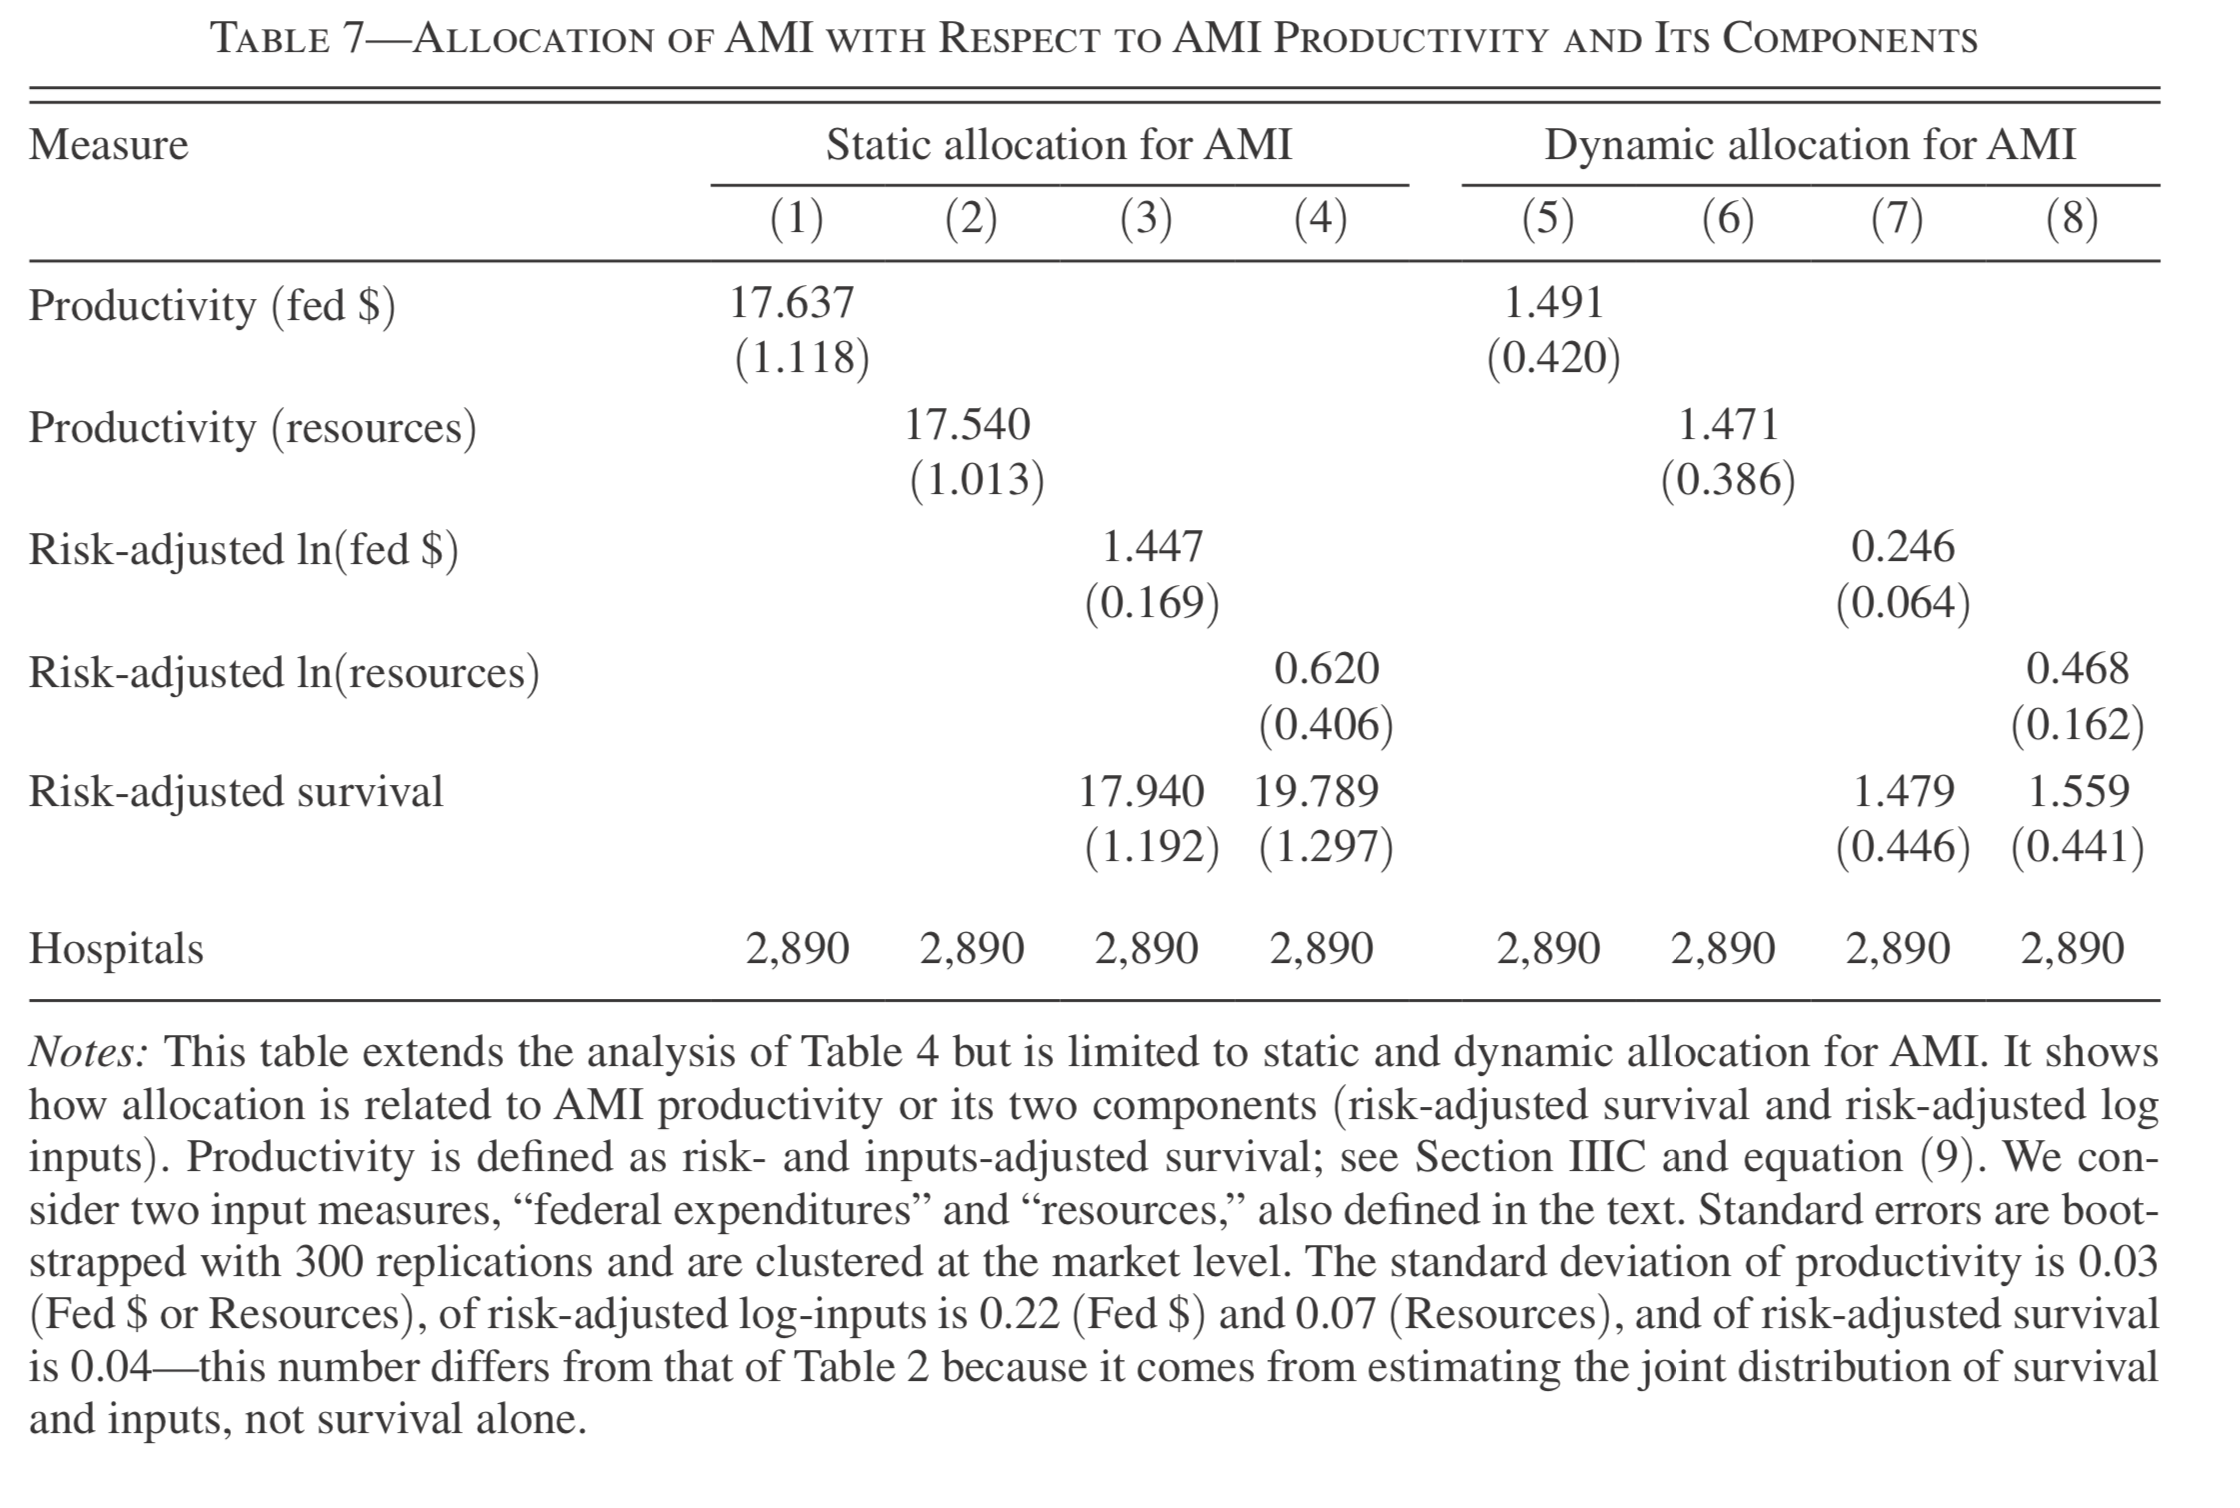
\includegraphics[width=4in]{./resources/hc7.png}
\end{center}
\end{frame}

\begin{frame}{Healthcare Exceptionalism: EB Adjustment}
\begin{center}
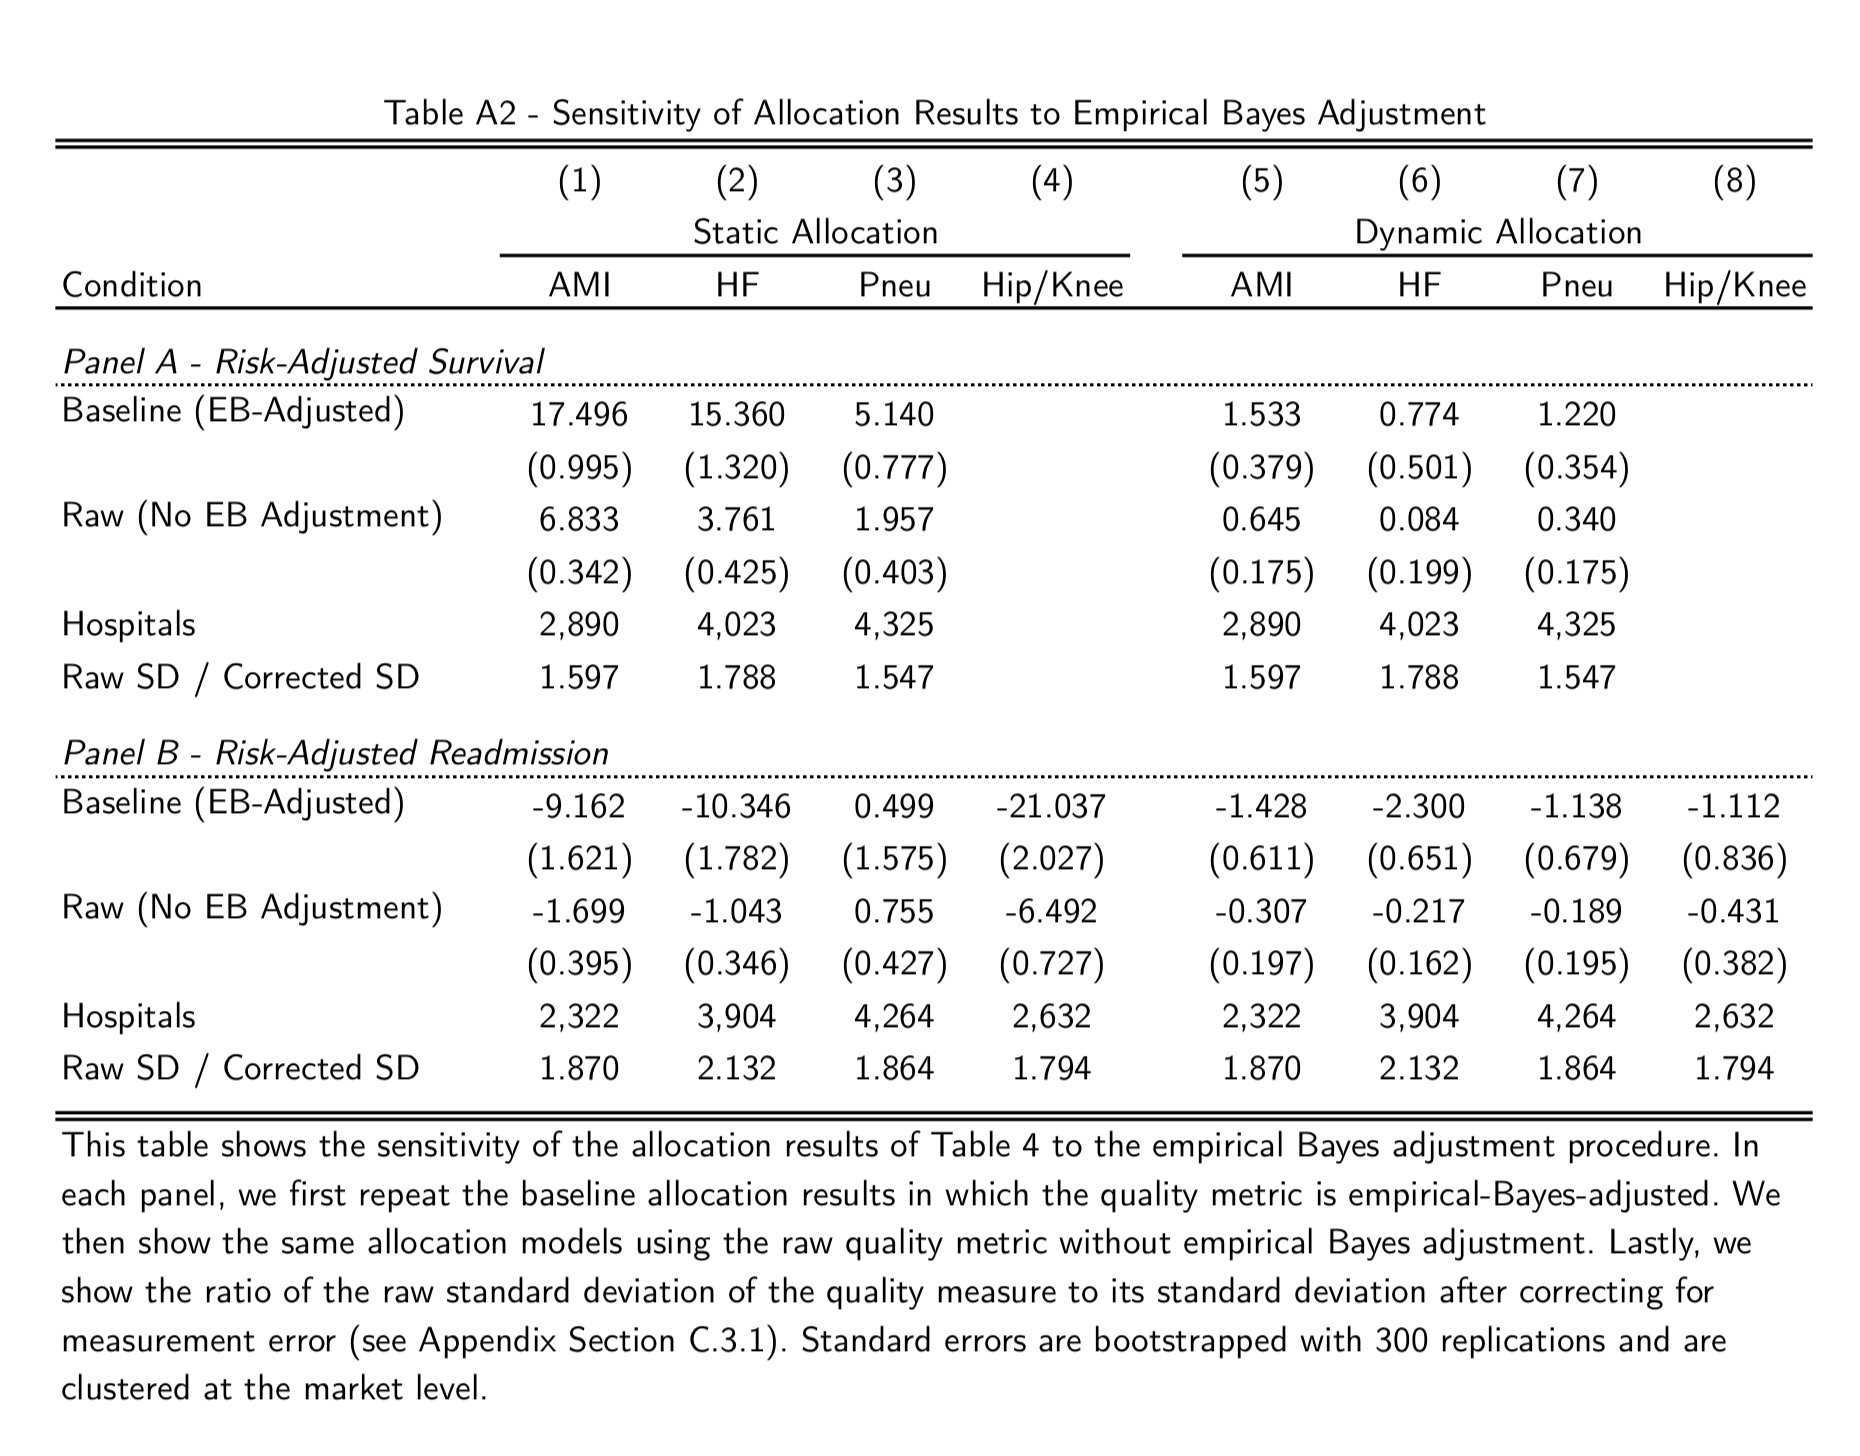
\includegraphics[width=4in]{./resources/hc_a2.png}
\end{center}
\end{frame}


\section*{Thanks!}




\end{document}